Implementiamo in questo esercizio un multiclass classification problem con un Decision Tree.
Iniziamo dal caso binario lo estendiamo al problema multiclasse.

Il parametro da ottimizzare in questo problema può essere la depth dell'albero. Anche in questo caso dividiamo il dataset in due insiemi, il learning set e il validation set e usando il validation set calcoliamo l'errore come numero di punti classificati in modo errato. Anche qui reiteriamo il prodcedimento k volte, con k uguale a 30.

In this exercise we implement a multiclass classification problem with a Decision Tree.
We start from the binary case and extend it to the multiclass problem.

The parameter to be optimized in this problem can be the depth of the tree. Also in this case we divide the dataset into two sets, the learning set and the validation set and using the validation set we calculate the error as the number of points classified incorrectly. Here again we repeat the product k times, with k equal to 30.

	\begin{figure}[h]
	\centering
	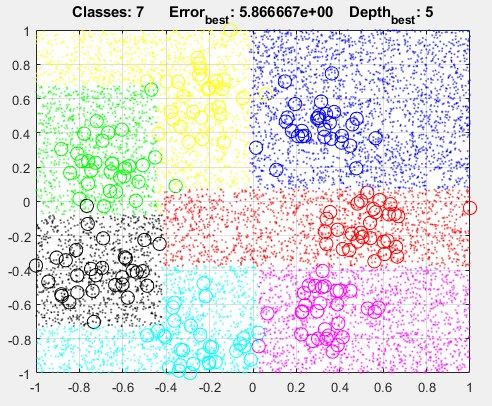
\includegraphics[width=0.5\textwidth]{i3.png}
	\caption{Regression Function}
	\label{fig:regression function}
\end{figure}